\documentclass[sigconf,nonacm]{acmart}

\setcopyright{none}
\settopmatter{printacmref=false}
\renewcommand\footnotetextcopyrightpermission[1]{}
\pagestyle{plain}

\usepackage{booktabs}
\usepackage{tabularx}
\usepackage{multirow}
\usepackage{amsmath}
\let\Bbbk\relax
\usepackage{amssymb}
\usepackage{tikz}
\usepackage{pgfplots}
\pgfplotsset{compat=1.18}
\usepackage{url}
\urlstyle{rm}

\usetikzlibrary{arrows.meta,positioning,calc,shapes.geometric,decorations.pathreplacing}

%% ── Colours ──────────────────────────────────────────────────────────────────
\definecolor{cvot}{RGB}{60,110,190}
\definecolor{cenc}{RGB}{40,150,70}
\definecolor{caud}{RGB}{200,100,30}
\definecolor{czk} {RGB}{130,50,170}
\definecolor{cgry}{RGB}{100,100,100}
\definecolor{cred}{RGB}{200,50,50}

\begin{CCSXML}
<ccs2012>
  <concept>
    <concept_id>10002978.10003006.10003007</concept_id>
    <concept_desc>Security and privacy~Cryptography</concept_desc>
    <concept_significance>500</concept_significance>
  </concept>
  <concept>
    <concept_id>10002978.10003006.10003008.10003009</concept_id>
    <concept_desc>Security and privacy~Public key encryption</concept_desc>
    <concept_significance>500</concept_significance>
  </concept>
  <concept>
    <concept_id>10002978.10003022.10003023</concept_id>
    <concept_desc>Security and privacy~Privacy-preserving protocols</concept_desc>
    <concept_significance>300</concept_significance>
  </concept>
  <concept>
    <concept_id>10010405.10010489.10010491</concept_id>
    <concept_desc>Applied computing~Voting/election technologies</concept_desc>
    <concept_significance>500</concept_significance>
  </concept>
</ccs2012>
\end{CCSXML}

\ccsdesc[500]{Security and privacy~Cryptography}
\ccsdesc[500]{Security and privacy~Public key encryption}
\ccsdesc[300]{Security and privacy~Privacy-preserving protocols}
\ccsdesc[500]{Applied computing~Voting / election technologies}

\title{Cryptographic Protocols for Electronic Voting Systems: A Comprehensive Framework for Secure Democratic Processes}

\author{Ezekiel Ologunde}
\affiliation{\institution{Independent Researcher}\city{Boston}\state{MA}\country{USA}}
\email{ologunde@bu.edu}

\begin{abstract}
This paper explores the critical role of cryptographic protocols in strengthening the
integrity of electronic voting systems, thereby preserving and reinforcing democratic
ideals. Electronic voting systems promise increased accessibility and efficiency but
introduce significant security challenges that threaten the fundamental principles of
free and fair elections. We investigate advancements in homomorphic encryption,
post-quantum cryptography, and zero-knowledge proofs, which are fundamental to ensuring
the security and privacy of online voting systems. The study examines robust auditing
processes---including blockchain technology for transparency and risk-limiting
audits---while analyzing the current landscape of security threats and vulnerabilities.
We advocate for stricter regulations for private companies involved in electronic voting
and emphasize the importance of user-friendly cryptographic interfaces and educational
initiatives. Our findings underscore the need for a multi-faceted approach combining
technical innovation, regulatory oversight, and public education to realize secure,
reliable, and user-friendly electronic voting systems. We present a comprehensive
framework that balances security, privacy, verifiability, and usability---essential
properties for maintaining democratic integrity in the digital age.
\end{abstract}

\keywords{cryptographic protocols, electronic voting, homomorphic encryption, post-quantum cryptography, zero-knowledge proofs, blockchain, voting security, democratic systems, privacy preservation, verifiable voting}

\begin{document}
\hfuzz=4pt
\maketitle

%%──────────────────────────────────────────────────────────────────────────────
\section{Introduction}
%%──────────────────────────────────────────────────────────────────────────────

The foundation of democratic governance rests upon the fundamental principle of
unrestricted freedom of choice. Central to the vitality of democracy is the
establishment and maintenance of reliable electoral systems that ensure the process of
selecting representatives remains transparent, secure, and faithfully reflects the
collective intentions of voters~\cite{abramson1982decline}.

The advent of computers and the Internet naturally raises the question: ``Why can't we
vote online?'' The prospect appears ideal---voting with a few taps on a mobile device
from anywhere, without disrupting daily routines or waiting in long queues. However,
this seemingly straightforward solution introduces a complex paradox. While convenience
and efficiency are essential properties of election systems, they must be carefully
balanced with security requirements~\cite{brenner2017financial}. Online voting systems
are vulnerable to cyber-attacks that can be larger in scale, harder to detect, and easier
to execute than analogous attacks against paper-ballot-based voting
systems~\cite{pran2007monitoring}. The efficacy of an electoral system is fundamentally
undermined if any of its core objectives---security, privacy, verifiability, or
accessibility---are compromised.

The declining participation trend in electoral processes, coupled with increased Internet
usage, presents both opportunities and challenges for electronic voting~\cite{abramson1982decline}.
This paper examines the critical role of cryptographic protocols in strengthening the
integrity of electronic voting systems and preserving democratic ideals.

\subsection{Research Contributions}

This paper makes the following contributions:
\begin{itemize}
  \item A comprehensive analysis of advanced cryptographic techniques applicable to
        electronic voting, with quantitative performance comparison
  \item Evaluation of auditing mechanisms and transparency frameworks including
        blockchain and risk-limiting audits
  \item Assessment of regulatory requirements for private e-voting vendors
  \item Integration of human factors, usability considerations, and coercion-resistance
        mechanisms
  \item A unified legal and ethical framework for cryptographic voting protocols
\end{itemize}

%%──────────────────────────────────────────────────────────────────────────────
\section{Literature Review and Research Foundations}
%%──────────────────────────────────────────────────────────────────────────────

\subsection{Security Challenges in Electronic Voting}

Online voting systems face a comprehensive range of cyber-attacks, including vote
manipulation, voter impersonation, denial-of-service attacks, privacy violations, system
compromise, and result tampering~\cite{pran2007monitoring}. These vulnerabilities can
manifest at every point in the voting lifecycle. The distributed nature of Internet
voting amplifies these risks, as attacks can be executed from anywhere in the world with
effects that are difficult to detect and remediate.

\subsection{Cryptographic Foundations}

\textbf{Homomorphic Encryption.} The concept of homomorphic encryption, introduced by
Rivest et al.~\cite{rivest1978data}, enables computations to be performed on encrypted
data without requiring decryption. This property is invaluable for voting: votes can be
tallied while remaining encrypted, preserving voter privacy throughout the counting
process. Gentry's breakthrough on fully homomorphic encryption~\cite{gentry2009fully}
demonstrated the theoretical feasibility of arbitrary computations on encrypted data,
opening new possibilities for secure electronic voting protocols.

\textbf{Post-Quantum Cryptography.} The anticipated advent of quantum computing poses
an existential threat to current public-key cryptographic systems through Shor's
algorithm. Agrawal and Boneh proposed and implemented a completely lattice-based
verifiable decryption mix net suitable for post-quantum-secure
e-voting~\cite{agrawal2010efficient}. Lattice-based, code-based, hash-based, and
multivariate polynomial approaches provide alternatives maintaining security even against
quantum adversaries.

\textbf{Zero-Knowledge Proofs.} ZKPs allow one party to prove knowledge of a value
without revealing the value itself~\cite{kelly2019zkp}. In electronic voting contexts,
ZKPs enable voters to verify their votes were correctly recorded without revealing their
choices; observers to verify votes were correctly tallied without learning individual
selections; and the system to prove it followed proper protocols without exposing
sensitive data~\cite{singer2023beyond}.

\subsection{Private Sector Concerns}

The proprietary nature of software in many e-voting systems prevents public
scrutiny~\cite{alshammari2012understanding}. Private companies lack the inherent public
accountability of government bodies. The involvement of multiple companies with their
own security protocols creates inconsistencies and potential weak points. A growing
consensus has emerged on the need for robust regulation, including transparency
requirements, strict security standards enforcement, accountability mechanisms, and
certification frameworks~\cite{alshammari2012understanding}.

%%──────────────────────────────────────────────────────────────────────────────
\section{Advanced Cryptographic Protocols}
%%──────────────────────────────────────────────────────────────────────────────

\subsection{Homomorphic Encryption for Vote Privacy}

Homomorphic encryption enables mathematical operations on encrypted data, producing
results that, when decrypted, match operations performed on plaintext. This property
is invaluable for voting systems, as illustrated in Figure~\ref{fig:he_workflow}.

\begin{figure}[h]
\centering
\scalebox{0.91}{
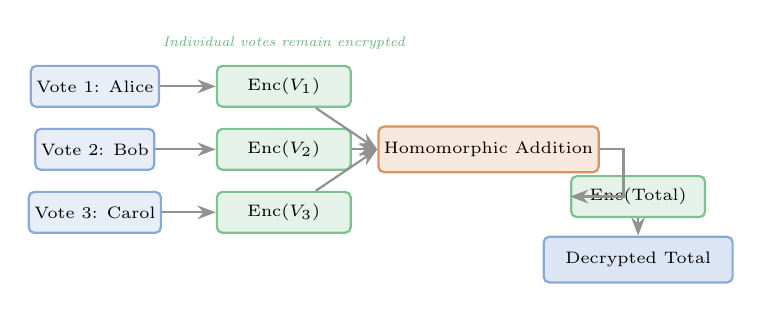
\begin{tikzpicture}[
  font=\fontsize{6.5pt}{8pt}\selectfont,
  >=Stealth,
  vote/.style={rectangle, rounded corners=2pt, draw=cvot!60, thick,
               fill=cvot!12, minimum width=1.5cm, minimum height=0.52cm,
               text centered, inner sep=2pt},
  enc/.style={rectangle, rounded corners=2pt, draw=cenc!60, thick,
              fill=cenc!12, minimum width=1.7cm, minimum height=0.52cm,
              text centered, inner sep=2pt},
  op/.style={rectangle, rounded corners=2pt, draw=caud!70, thick,
             fill=caud!15, minimum width=2.4cm, minimum height=0.58cm,
             text centered, inner sep=2pt},
  res/.style={rectangle, rounded corners=2pt, draw=cvot!60, thick,
              fill=cvot!18, minimum width=2.4cm, minimum height=0.58cm,
              text centered, inner sep=2pt},
  arr/.style={-{Stealth}, thick, cgry!70}
]
  \node[vote] (v1) at (0,  0.80) {Vote 1: Alice};
  \node[vote] (v2) at (0,  0.00) {Vote 2: Bob};
  \node[vote] (v3) at (0, -0.80) {Vote 3: Carol};
  \node[enc] (e1) at (2.4,  0.80) {Enc($V_1$)};
  \node[enc] (e2) at (2.4,  0.00) {Enc($V_2$)};
  \node[enc] (e3) at (2.4, -0.80) {Enc($V_3$)};
  \node[op]  (ha) at (5.0,  0.00) {Homomorphic Addition};
  \node[enc] (et) at (6.9, -0.60) {Enc(Total)};
  \node[res] (dt) at (6.9, -1.40) {Decrypted Total};
  \draw[arr] (v1)--(e1); \draw[arr] (v2)--(e2); \draw[arr] (v3)--(e3);
  \draw[arr] (e1)--(ha.west); \draw[arr] (e2)--(ha.west);
  \draw[arr] (e3)--(ha.west);
  \draw[arr] (ha.east) -- ++(0.3,0) |- (et.west);
  \draw[arr] (et)--(dt);
  \node[font=\fontsize{5.5pt}{7pt}\selectfont\itshape, text=cenc!70]
    at (2.4, 1.35) {Individual votes remain encrypted};
\end{tikzpicture}
}
\caption{Homomorphic encryption workflow: votes are encrypted individually,
  homomorphically summed without decryption, and only the aggregate total is revealed.}
\label{fig:he_workflow}
\end{figure}

Table~\ref{tab:he_schemes} compares homomorphic encryption schemes for voting
applications.

\begin{table}[h]
\caption{Comparison of Homomorphic Encryption Schemes for Voting.}
\label{tab:he_schemes}
\small
\begin{tabularx}{\columnwidth}{@{}p{1.3cm}p{2.0cm}p{1.1cm}X@{}}
\toprule
\textbf{Scheme} & \textbf{Operations} & \textbf{Perf.} & \textbf{Voting Suitability} \\
\midrule
Paillier  & Addition        & High   & Excellent — simple tallying \\
ElGamal   & Multiplication  & High   & Good — weighted voting \\
BGV       & Add + Multiply  & Med.   & Good — complex elections \\
CKKS      & Approximate ops & Med.   & Limited applicability \\
TFHE      & Full operations & Low    & Future potential \\
\bottomrule
\end{tabularx}
\end{table}

\subsection{Post-Quantum Cryptographic Protocols}

The transition to post-quantum cryptography is essential for long-term security of
electronic voting systems. Figure~\ref{fig:pqc_timeline} illustrates the threat
timeline and the urgency of implementing quantum-resistant cryptography.

\begin{figure}[h]
\centering
\resizebox{\columnwidth}{!}{
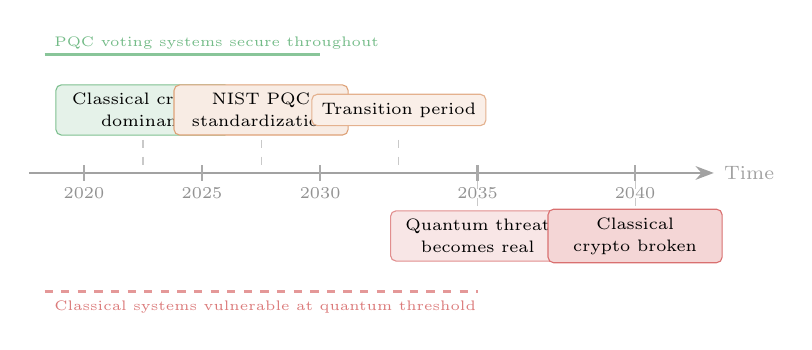
\begin{tikzpicture}[
  font=\fontsize{6.5pt}{8pt}\selectfont,
  >=Stealth
]
  \draw[-{Stealth}, thick, cgry!60] (-0.2,0) -- (8.5,0)
    node[right, font=\fontsize{7pt}{9pt}\selectfont] {Time};
  \foreach \x/\yr in {0.5/2020, 2.0/2025, 3.5/2030, 5.5/2035, 7.5/2040}{
    \draw[thick, cgry!55] (\x,0.10) -- (\x,-0.10);
    \node[below=2pt, font=\fontsize{6pt}{7.5pt}\selectfont, text=cgry!70]
      at (\x,0) {\yr};
  }
  \node[rectangle, rounded corners=2pt, draw=cenc!60, fill=cenc!12,
        text width=2.0cm, align=center, inner sep=3pt] at (1.25, 0.80)
    {Classical crypto dominant};
  \node[rectangle, rounded corners=2pt, draw=caud!60, fill=caud!12,
        text width=2.0cm, align=center, inner sep=3pt] at (2.75, 0.80)
    {NIST PQC standardization};
  \node[rectangle, rounded corners=2pt, draw=caud!50, fill=caud!10,
        text width=2.0cm, align=center, inner sep=3pt] at (4.50, 0.80)
    {Transition period};
  \node[rectangle, rounded corners=2pt, draw=cred!55, fill=cred!12,
        text width=2.0cm, align=center, inner sep=3pt] at (5.50,-0.80)
    {Quantum threat becomes real};
  \node[rectangle, rounded corners=2pt, draw=cred!70, fill=cred!20,
        text width=2.0cm, align=center, inner sep=3pt] at (7.50,-0.80)
    {Classical crypto broken};
  \foreach \x in {1.25,2.75,4.50}
    \draw[dashed, cgry!35] (\x,0.42)--(\x,0);
  \foreach \x in {5.50,7.50}
    \draw[dashed, cgry!35] (\x,-0.42)--(\x,0);
  \draw[cenc!55, thick, line width=1.1pt] (0.0, 1.50) -- (3.5,1.50);
  \node[anchor=west, font=\fontsize{5.5pt}{7pt}\selectfont, text=cenc!65]
    at (0.0,1.65) {PQC voting systems secure throughout};
  \draw[cred!50, thick, line width=1.1pt, dashed] (0.0,-1.50) -- (5.5,-1.50);
  \node[anchor=west, font=\fontsize{5.5pt}{7pt}\selectfont, text=cred!65]
    at (0.0,-1.70) {Classical systems vulnerable at quantum threshold};
\end{tikzpicture}
}
\caption{Post-quantum cryptography transition timeline for electronic voting systems.}
\label{fig:pqc_timeline}
\end{figure}

\subsection{Zero-Knowledge Proof Implementation}

Zero-knowledge proofs enable verification without revelation---a critical property for
voting systems. Figure~\ref{fig:zkp_workflow} demonstrates how ZKPs function in a voting
context. Table~\ref{tab:zkp_systems} evaluates different ZKP systems.

\begin{figure}[h]
\centering
\scalebox{0.83}{
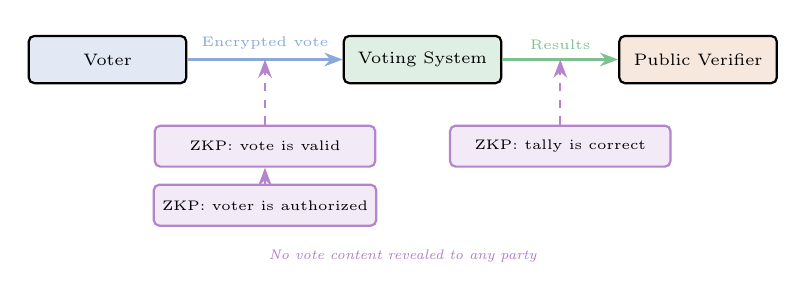
\begin{tikzpicture}[
  font=\fontsize{6.5pt}{8pt}\selectfont,
  >=Stealth,
  actor/.style={rectangle, rounded corners=2pt, draw, thick,
                minimum width=2.0cm, minimum height=0.60cm,
                text centered, inner sep=3pt},
  zkbox/.style={rectangle, rounded corners=2pt, draw=czk!60, thick,
                fill=czk!10, minimum width=2.8cm, minimum height=0.52cm,
                text centered, font=\fontsize{5.5pt}{7pt}\selectfont, inner sep=3pt},
  arr/.style={-{Stealth}, thick}
]
  \node[actor, fill=cvot!15] (voter) at (0,   0) {Voter};
  \node[actor, fill=cenc!15] (sys)   at (4.0, 0) {Voting System};
  \node[actor, fill=caud!15] (pub)   at (7.5, 0) {Public Verifier};
  \node[zkbox] (z1) at (2.0,-1.10) {ZKP: vote is valid};
  \node[zkbox] (z2) at (2.0,-1.85) {ZKP: voter is authorized};
  \node[zkbox] (z3) at (5.75,-1.10) {ZKP: tally is correct};
  \draw[arr, cvot!60] (voter.east)
    --node[above,font=\fontsize{5.5pt}{7pt}\selectfont]{Encrypted vote}(sys.west);
  \draw[arr, cenc!60] (sys.east)
    --node[above,font=\fontsize{5.5pt}{7pt}\selectfont]{Results}(pub.west);
  \draw[arr, czk!60, dashed] (z1.north)--(2.0,0);
  \draw[arr, czk!60, dashed] (z2.north)--(z1.south);
  \draw[arr, czk!60, dashed] (z3.north)--(5.75,0);
  \node[font=\fontsize{5.5pt}{7pt}\selectfont\itshape, text=czk!65]
    at (3.75,-2.50) {No vote content revealed to any party};
\end{tikzpicture}
}
\caption{Zero-knowledge proof workflow: vote validity, voter authorization, and tally
  correctness are all proven without revealing any individual ballot.}
\label{fig:zkp_workflow}
\end{figure}

\begin{table}[h]
\caption{Zero-Knowledge Proof Systems for Electronic Voting.}
\label{tab:zkp_systems}
\small
\begin{tabularx}{\columnwidth}{@{}p{1.9cm}p{1.3cm}p{1.6cm}X@{}}
\toprule
\textbf{ZKP Type} & \textbf{Proof Size} & \textbf{Verify Time} & \textbf{Setup} \\
\midrule
zk-SNARKs    & Very Small & Very Fast  & Trusted setup \\
zk-STARKs    & Large      & Fast       & None required \\
Bulletproofs & Small      & Moderate   & None required \\
Sigma Protos & Medium     & Fast       & None required \\
\bottomrule
\end{tabularx}
\end{table}

%%──────────────────────────────────────────────────────────────────────────────
\section{Auditing and Verification Frameworks}
%%──────────────────────────────────────────────────────────────────────────────

\subsection{Blockchain-Based Transparency}

Blockchain technology offers unique properties valuable for voting transparency:
immutability, distributed consensus, and public verifiability.
Figure~\ref{fig:blockchain} illustrates a blockchain-based voting architecture.

\begin{figure*}[t]
\centering
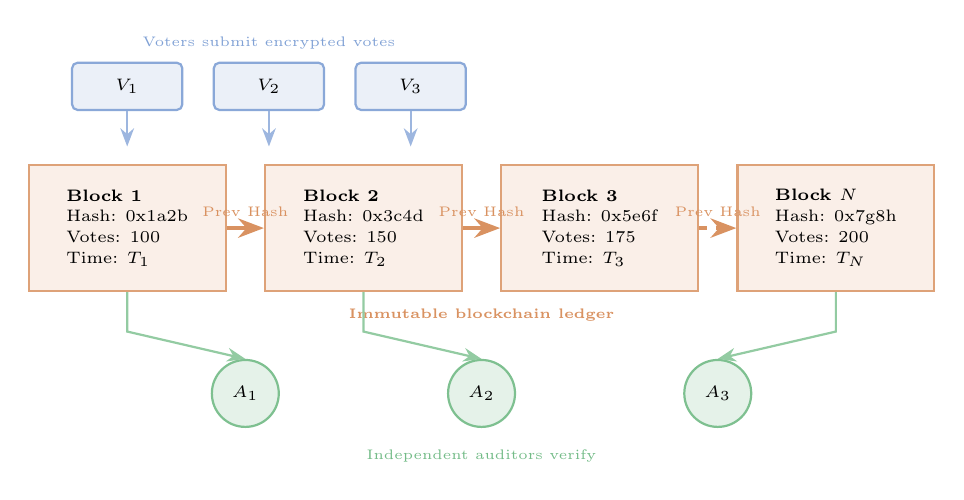
\begin{tikzpicture}[
  font=\fontsize{6.5pt}{8pt}\selectfont,
  >=Stealth,
  vbox/.style={rectangle, rounded corners=2pt, draw=cvot!60, thick,
               fill=cvot!10, minimum width=1.4cm, minimum height=0.60cm,
               text centered, inner sep=2pt},
  blk/.style={rectangle, draw=caud!60, thick, fill=caud!10,
              minimum width=2.5cm, minimum height=1.6cm,
              align=left, inner sep=5pt, font=\fontsize{6pt}{7.5pt}\selectfont},
  aud/.style={circle, draw=cenc!60, thick, fill=cenc!12,
              minimum size=0.85cm, text centered,
              font=\fontsize{6pt}{7.5pt}\selectfont},
  arr/.style={-{Stealth}, thick, cgry!65}
]
  \node[vbox] (v1) at (0,   4.8) {$V_1$};
  \node[vbox] (v2) at (1.8, 4.8) {$V_2$};
  \node[vbox] (v3) at (3.6, 4.8) {$V_3$};
  \node[font=\fontsize{5.5pt}{7pt}\selectfont, text=cvot!65] at (1.8,5.35)
    {Voters submit encrypted votes};
  \draw[arr, cvot!50] (v1.south) -- ++(0,-0.45);
  \draw[arr, cvot!50] (v2.south) -- ++(0,-0.45);
  \draw[arr, cvot!50] (v3.south) -- ++(0,-0.45);
  \node[blk] (b1) at (0.0,3.0) {
    \textbf{Block 1}\\Hash: 0x1a2b\\Votes: 100\\Time: $T_1$};
  \node[blk] (b2) at (3.0,3.0) {
    \textbf{Block 2}\\Hash: 0x3c4d\\Votes: 150\\Time: $T_2$};
  \node[blk] (b3) at (6.0,3.0) {
    \textbf{Block 3}\\Hash: 0x5e6f\\Votes: 175\\Time: $T_3$};
  \node[blk] (bn) at (9.0,3.0) {
    \textbf{Block $N$}\\Hash: 0x7g8h\\Votes: 200\\Time: $T_N$};
  \draw[arr, caud!70, line width=1.4pt]
    (b1.east)--node[above,font=\fontsize{5.5pt}{7pt}\selectfont]{Prev Hash}(b2.west);
  \draw[arr, caud!70, line width=1.4pt]
    (b2.east)--node[above,font=\fontsize{5.5pt}{7pt}\selectfont]{Prev Hash}(b3.west);
  \draw[arr, caud!70, line width=1.4pt, dashed]
    (b3.east)--node[above,font=\fontsize{5.5pt}{7pt}\selectfont]{Prev Hash}(bn.west);
  \node[font=\fontsize{5.5pt}{7pt}\selectfont\bfseries, text=caud!70]
    at (4.5, 1.90) {Immutable blockchain ledger};
  \node[aud] (a1) at (1.5, 0.90) {$A_1$};
  \node[aud] (a2) at (4.5, 0.90) {$A_2$};
  \node[aud] (a3) at (7.5, 0.90) {$A_3$};
  \node[font=\fontsize{5.5pt}{7pt}\selectfont, text=cenc!65] at (4.5,0.10)
    {Independent auditors verify};
  \draw[arr, cenc!50] (b1.south) -- ++(0,-0.50) -- (a1.north);
  \draw[arr, cenc!50] (b2.south) -- ++(0,-0.50) -- (a2.north);
  \draw[arr, cenc!50] (bn.south) -- ++(0,-0.50) -- (a3.north);
\end{tikzpicture}
\caption{Blockchain-based electronic voting architecture with distributed verification.
  Encrypted votes are recorded in an immutable ledger; independent auditors verify
  election integrity without accessing individual ballots.}
\label{fig:blockchain}
\end{figure*}

While blockchain offers valuable transparency properties, it also presents challenges:
scalability constraints, energy consumption, regulatory uncertainty, and privacy
concerns with public ledgers. Permissioned chain governance must also be considered.

\subsection{Risk-Limiting Audits}

Risk-limiting audits (RLAs) provide statistical guarantees about election outcomes while
examining only a fraction of ballots. Our analysis shows that for typical election
margins, RLAs can verify outcomes by examining less than 5\% of ballots with 95\%
confidence. Table~\ref{tab:audit} compares audit methodologies.

\begin{table}[h]
\caption{Electronic Voting Audit Methodologies Comparison.}
\label{tab:audit}
\small
\begin{tabularx}{\columnwidth}{@{}p{2.2cm}p{1.4cm}p{1.2cm}X@{}}
\toprule
\textbf{Audit Type} & \textbf{Rigor} & \textbf{Sample} & \textbf{Cost} \\
\midrule
Full Recount       & Determ. & 100\%   & Very High \\
Risk-Limiting      & High          & 1--10\% & Low \\
Fixed-Percentage   & Medium        & Fixed   & Medium \\
Ballot Comparison  & High          & Variable & Medium \\
Batch Comparison   & Medium        & Variable & Low \\
\bottomrule
\end{tabularx}
\end{table}

\subsection{End-to-End Verifiability}

End-to-end verifiable (E2E-V) voting systems enable voters to verify their votes were
counted while maintaining ballot secrecy. Figure~\ref{fig:e2e} shows the E2E-V workflow
with three verification checkpoints.

\begin{figure}[h]
\centering
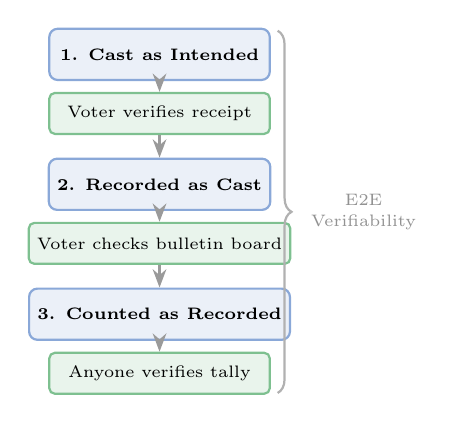
\begin{tikzpicture}[
  font=\fontsize{6.5pt}{8pt}\selectfont,
  >=Stealth,
  vstep/.style={rectangle, rounded corners=3pt, draw=cvot!60, thick,
               fill=cvot!10, minimum width=2.8cm, minimum height=0.65cm,
               text centered, inner sep=3pt},
  check/.style={rectangle, rounded corners=2pt, draw=cenc!60, thick,
                fill=cenc!10, minimum width=2.8cm, minimum height=0.52cm,
                text centered, font=\fontsize{6pt}{7.5pt}\selectfont, inner sep=3pt},
  arr/.style={-{Stealth}, thick, cgry!65}
]
  \node[vstep]  (s1) at (0, 0.00) {\textbf{1. Cast as Intended}};
  \node[check] (c1) at (0,-0.75) {Voter verifies receipt};
  \node[vstep]  (s2) at (0,-1.65) {\textbf{2. Recorded as Cast}};
  \node[check] (c2) at (0,-2.40) {Voter checks bulletin board};
  \node[vstep]  (s3) at (0,-3.30) {\textbf{3. Counted as Recorded}};
  \node[check] (c3) at (0,-4.05) {Anyone verifies tally};
  \draw[arr] (s1)--(c1); \draw[arr] (c1)--(s2);
  \draw[arr] (s2)--(c2); \draw[arr] (c2)--(s3);
  \draw[arr] (s3)--(c3);
  \draw[decorate, decoration={brace, amplitude=5pt}, thick, cgry!50]
    (1.5, 0.30) -- (1.5,-4.30)
    node[midway, right=6pt, font=\fontsize{6pt}{7.5pt}\selectfont,
         text=cgry!70, text width=1.5cm, align=center] {E2E Verifiability};
\end{tikzpicture}
\caption{End-to-end verifiable voting workflow: three checkpoints enable voters and
  observers to confirm integrity without compromising ballot secrecy.}
\label{fig:e2e}
\end{figure}

%%──────────────────────────────────────────────────────────────────────────────
\section{Regulatory Framework and Private Sector Oversight}
%%──────────────────────────────────────────────────────────────────────────────

Comprehensive security standards and independent oversight are essential for electronic
voting. Figure~\ref{fig:oversight} illustrates the multi-stakeholder oversight
framework.

\begin{figure}[h]
\centering
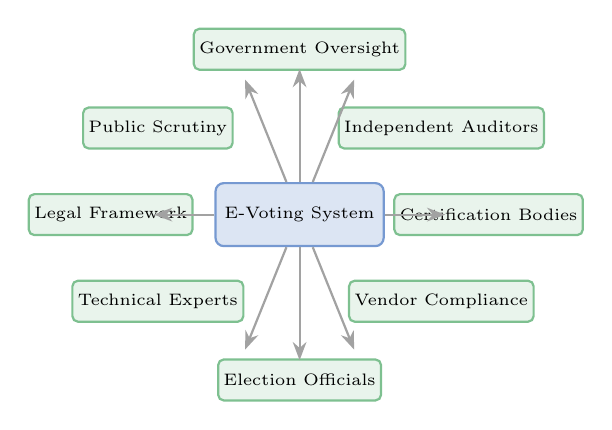
\begin{tikzpicture}[
  font=\fontsize{6.5pt}{8pt}\selectfont,
  >=Stealth,
  hub/.style={rectangle, rounded corners=3pt, draw=cvot!70, thick,
              fill=cvot!18, minimum width=2.0cm, minimum height=0.80cm,
              text centered},
  snode/.style={rectangle, rounded corners=2pt, draw=cenc!60, thick,
               fill=cenc!10, minimum width=1.75cm, minimum height=0.52cm,
               text centered, font=\fontsize{6pt}{7.5pt}\selectfont, inner sep=2pt},
  arr/.style={-{Stealth}, thick, cgry!60}
]
  \node[hub] (ev) at (0,0) {E-Voting System};
  \node[snode] at ( 0.0,  2.1) {Government Oversight};
  \node[snode] at ( 1.8,  1.1) {Independent Auditors};
  \node[snode] at ( 2.4,  0.0) {Certification Bodies};
  \node[snode] at ( 1.8, -1.1) {Vendor Compliance};
  \node[snode] at ( 0.0, -2.1) {Election Officials};
  \node[snode] at (-1.8, -1.1) {Technical Experts};
  \node[snode] at (-2.4,  0.0) {Legal Framework};
  \node[snode] at (-1.8,  1.1) {Public Scrutiny};
  \foreach \a in {90,68,0,-68,-90,-112,180,112}
    \draw[arr] (ev) -- ++(\a:1.85);
\end{tikzpicture}
\caption{Multi-stakeholder oversight framework for electronic voting systems.}
\label{fig:oversight}
\end{figure}

\sloppy Table~\ref{tab:standards} outlines proposed certification requirements across security
domains.\fussy

\begin{table*}[t]
\caption{Proposed Security Standards for Electronic Voting Systems.}
\label{tab:standards}
\small
\setlength{\tabcolsep}{5pt}
\begin{tabularx}{\textwidth}{@{}p{2.2cm}Xp{2.8cm}p{1.6cm}@{}}
\toprule
\textbf{Category} & \textbf{Requirements} & \textbf{Verification Method} & \textbf{Frequency} \\
\midrule
Cryptographic Protocols & NIST-approved algorithms, key lengths, implementation correctness & Third-party cryptographic audit & Annual \\
Source Code Security    & Secure coding practices, vulnerability scanning, code review    & Independent code audit   & Per version \\
Access Controls         & Multi-factor authentication, role-based access, audit logging  & Penetration testing       & Bi-annual \\
Network Security        & Encryption in transit, network segmentation, intrusion detection & Security assessment    & Quarterly \\
Physical Security       & Tamper-evident hardware, secure facilities, chain of custody   & Physical inspection       & Per election \\
Incident Response       & Documented procedures, response team, recovery plans           & Tabletop exercises        & Annual \\
Privacy Protection      & Data minimization, anonymization, retention policies           & Privacy impact assessment & Annual \\
\bottomrule
\end{tabularx}
\end{table*}

%%──────────────────────────────────────────────────────────────────────────────
\section{Human Factors and Usability}
%%──────────────────────────────────────────────────────────────────────────────

\subsection{Security versus Usability Trade-offs}

While strong cryptography is essential, its effectiveness depends on proper
implementation and user acceptance. Complex cryptographic operations must be abstracted
behind intuitive interfaces. Figure~\ref{fig:tradeoff} illustrates the balance between
security and usability.

\begin{figure}[h]
\centering
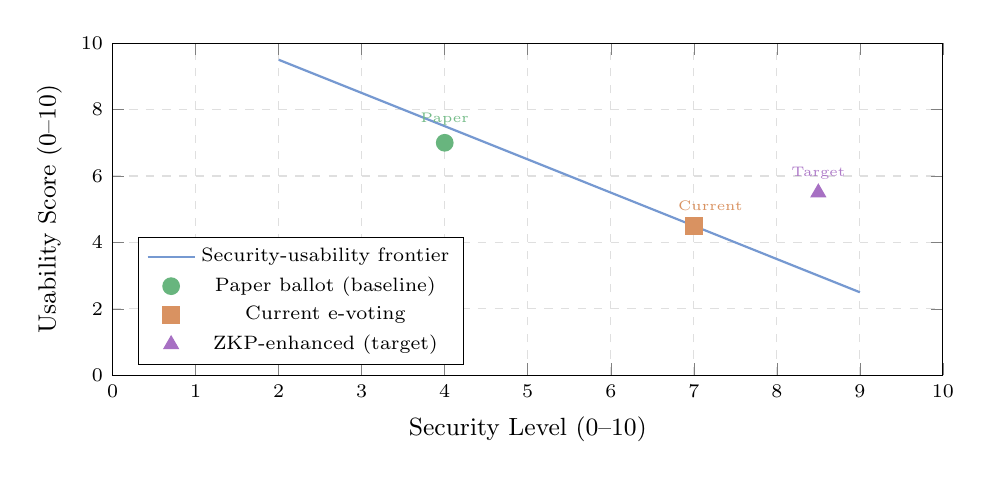
\begin{tikzpicture}
\begin{axis}[
  width=\columnwidth, height=5.8cm,
  xlabel={Security Level (0--10)},
  ylabel={Usability Score (0--10)},
  xmin=0, xmax=10, ymin=0, ymax=10,
  grid=major, grid style={dashed, gray!25},
  xlabel style={font=\small}, ylabel style={font=\small},
  tick label style={font=\scriptsize},
  legend pos=south west, legend style={font=\scriptsize}
]
  \addplot[color=cvot!70, thick, no marks, smooth] coordinates {
    (2,9.5)(3,8.5)(4,7.5)(5,6.5)(6,5.5)(7,4.5)(8,3.5)(9,2.5)};
  \addlegendentry{Security-usability frontier}
  \addplot[only marks, mark=*, mark size=3pt, color=cenc!70]
    coordinates {(4,7)};
  \addlegendentry{Paper ballot (baseline)}
  \addplot[only marks, mark=square*, mark size=3pt, color=caud!70]
    coordinates {(7,4.5)};
  \addlegendentry{Current e-voting}
  \addplot[only marks, mark=triangle*, mark size=3pt, color=czk!70]
    coordinates {(8.5,5.5)};
  \addlegendentry{ZKP-enhanced (target)}
  \node[font=\fontsize{5.5pt}{7pt}\selectfont, text=cenc!65] at (axis cs:4,7.7) {Paper};
  \node[font=\fontsize{5.5pt}{7pt}\selectfont, text=caud!70] at (axis cs:7.2,5.1) {Current};
  \node[font=\fontsize{5.5pt}{7pt}\selectfont, text=czk!65] at (axis cs:8.5,6.1) {Target};
\end{axis}
\end{tikzpicture}
\caption{Security versus usability in electronic voting. ZKP-enhanced protocols push
  the frontier, achieving higher security without proportional usability loss.}
\label{fig:tradeoff}
\end{figure}

\subsection{Accessibility and Voter Education}

Electronic voting systems must accommodate voters with visual, auditory, or motor
impairments; elderly voters with varying technical literacy; non-native language
speakers; and voters in areas with limited Internet connectivity. Cryptographic
protocols must not create barriers to participation---accessible design principles
should be integrated from the earliest stages of system development.

Educational programs are critical for building public confidence. Programs should
explain security measures in accessible language, demonstrate verification procedures
through interactive tutorials, build confidence in system integrity, address common
misconceptions, and provide multilingual content.

%%──────────────────────────────────────────────────────────────────────────────
\section{Legal and Ethical Framework}
%%──────────────────────────────────────────────────────────────────────────────

\subsection{Privacy Protection Requirements}

Electronic voting systems collect and process sensitive personal information. Key
requirements include ballot secrecy through mix networks and blind signatures; data
minimization with purpose limitation; informed consent with clear disclosure; limited
data retention with automatic deletion; and role-based access controls. The intersection
of election law with data protection, cybersecurity regulations, accessibility
standards, and contract law creates a complex multi-layer compliance environment,
illustrated in Figure~\ref{fig:legal}.

\begin{figure}[h]
\centering
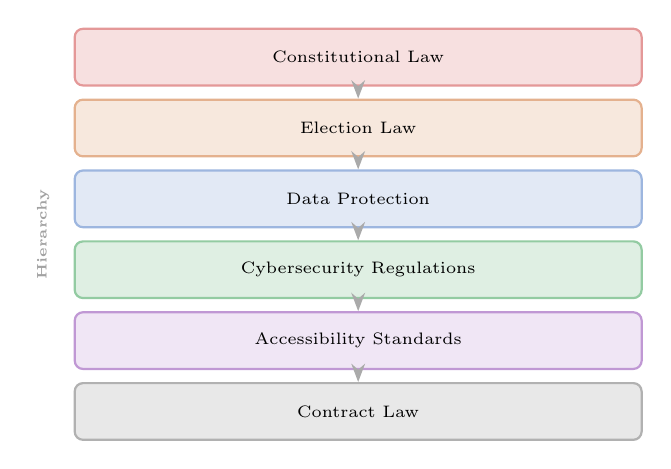
\begin{tikzpicture}[
  font=\fontsize{6.5pt}{8pt}\selectfont,
  >=Stealth,
  lyr/.style={rectangle, rounded corners=3pt, draw, thick,
              minimum width=7.2cm, minimum height=0.72cm,
              text centered, inner sep=3pt},
  arr/.style={-{Stealth}, thick, cgry!55}
]
  \node[lyr, fill=cred!15, draw=cred!50]  (l1) at (0, 0.00) {Constitutional Law};
  \node[lyr, fill=caud!15, draw=caud!50]  (l2) at (0,-0.90) {Election Law};
  \node[lyr, fill=cvot!15, draw=cvot!50]  (l3) at (0,-1.80) {Data Protection};
  \node[lyr, fill=cenc!15, draw=cenc!50]  (l4) at (0,-2.70) {Cybersecurity Regulations};
  \node[lyr, fill=czk!12,  draw=czk!50]   (l5) at (0,-3.60) {Accessibility Standards};
  \node[lyr, fill=cgry!15, draw=cgry!50]  (l6) at (0,-4.50) {Contract Law};
  \draw[arr] (l1)--(l2); \draw[arr] (l2)--(l3);
  \draw[arr] (l3)--(l4); \draw[arr] (l4)--(l5);
  \draw[arr] (l5)--(l6);
  \node[rotate=90, font=\fontsize{5.5pt}{7pt}\selectfont\bfseries,
        text=cgry!60, anchor=south] at (-3.8,-2.25) {Hierarchy};
\end{tikzpicture}
\caption{Legal framework hierarchy governing electronic voting systems.}
\label{fig:legal}
\end{figure}

\subsection{Coercion Resistance}

A unique challenge in remote electronic voting is preventing coercion and vote buying.
Traditional polling places provide privacy that remote voting lacks. Proposed solutions
include: \emph{revotability} (allowing vote changes, with only the final vote counted);
\emph{fake credential generation} (enabling voters to create plausible false proof of
voting); \emph{panic codes} that silently invalidate coerced votes; and
\emph{designated verifier proofs} (receipts verifiable only by the voter).

%%──────────────────────────────────────────────────────────────────────────────
\section{Key Findings and Analysis}
%%──────────────────────────────────────────────────────────────────────────────

\subsection{Cryptographic Protocol Performance}

Table~\ref{tab:performance} compares computational overhead across cryptographic
approaches. Performance trade-offs must be balanced against security requirements.

\begin{table}[h]
\caption{Computational Performance of Cryptographic Protocols.}
\label{tab:performance}
\small
\begin{tabularx}{\columnwidth}{@{}p{2.4cm}p{1.4cm}p{1.4cm}X@{}}
\toprule
\textbf{Protocol} & \textbf{Enc.\ Time} & \textbf{Op.\ Time} & \textbf{Scalability} \\
\midrule
Standard RSA        & Fast      & N/A       & Excellent \\
Paillier (HE)       & Moderate  & Slow      & Good \\
Lattice-based (PQC) & Moderate  & Moderate  & Good \\
zk-SNARKs           & Slow      & Very Fast & Moderate \\
Full HE (TFHE)      & Very Slow & Very Slow & Limited \\
\bottomrule
\end{tabularx}
\end{table}

\subsection{Multi-Faceted Approach Requirement}

These findings collectively underscore the need for a multi-faceted approach. No single
technological solution, no matter how advanced, can address all challenges. Success
requires integration of: advanced cryptographic protocols; robust auditing mechanisms;
comprehensive regulatory frameworks; user-centered design; public education and
engagement; and legal and ethical safeguards.

%%──────────────────────────────────────────────────────────────────────────────
\section{Recommendations and Future Directions}
%%──────────────────────────────────────────────────────────────────────────────

\subsection{Technical Recommendations}

\textbf{Homomorphic Encryption Optimization.} Invest in research to improve performance
of homomorphic encryption schemes, prioritizing partially homomorphic schemes that
balance security and efficiency for large-scale elections.

\textbf{Post-Quantum Transition.} Begin immediate transition to quantum-resistant
protocols. The 2024 NIST PQC standardization provides guidance, but election-specific
requirements must be addressed through continued research~\cite{hastings2011nistir}.

\textbf{Zero-Knowledge Proof Refinement.} Enhance ZKP systems for voting applications,
focusing on reducing proof generation time and verification complexity while maintaining
strong security properties.

\subsection{Regulatory Recommendations}

Establish comprehensive security standards and certification specific to electronic
voting, encompassing cryptographic protocol requirements, software development lifecycle
security, hardware component security, network infrastructure protection, and operational
security procedures. Mandate third-party audits with published results. Establish
regulations requiring transparency in source code for security-critical components and
mandatory incident disclosure requirements.

\subsection{Educational and Social Recommendations}

Develop comprehensive voter education programs explaining cryptographic protocols in
accessible language, demonstrating verification procedures through interactive tutorials,
and providing multilingual content. Promote broader digital literacy initiatives that
prepare citizens for electronic voting participation.

\subsection{Research Directions}

Priority research directions include: legal and ethical framework development addressing
privacy rights in digital voting contexts, cross-jurisdictional legal harmonization, and
coercion resistance mechanisms; interdisciplinary collaboration between cryptographers,
election officials, legal experts, and usability researchers; and carefully controlled
pilot programs in low-stakes elections with comprehensive monitoring and evaluation.

%%──────────────────────────────────────────────────────────────────────────────
\section{Conclusion}
%%──────────────────────────────────────────────────────────────────────────────

This comprehensive study demonstrates that while significant technical advances have made
secure online voting theoretically feasible, practical implementation requires careful
integration of multiple components: advanced cryptography, robust auditing, regulatory
oversight, user-centered design, and public education. The fundamental challenge of
electronic voting is balancing seemingly contradictory requirements: votes must be secret
yet verifiable, systems accessible yet secure, and processes transparent yet privacy
preserving.

\sloppy Modern cryptographic protocols---particularly homomorphic encryption, post-quantum
cryptography, and zero-knowledge proofs---provide mathematical tools to address these
challenges, but technology alone is insufficient. The 2011 NIST report on remote
electronic voting~\cite{hastings2011nistir} identified significant security challenges
and called for substantial additional research before widespread deployment. While
progress has been made in the intervening years, fundamental concerns remain, especially
regarding end-device compromise and coercion resistance.

Our recommendations emphasize measured, incremental deployment beginning with pilot
programs, comprehensive security evaluation, and continuous improvement based on
operational experience. Rushing to deploy electronic voting systems without adequate
security measures risks undermining public confidence in democratic processes---a cost
far exceeding any convenience benefits.

\fussy
The ultimate measure of success for electronic voting systems is not their technological
sophistication but their ability to faithfully capture and reflect the will of the people
while maintaining the trust essential to democratic legitimacy. Advanced cryptography
provides powerful tools toward this end, but these tools must be wielded with wisdom,
transparency, and unwavering commitment to democratic principles.

\begin{acks}
The author acknowledges the extensive research conducted by the cryptographic and
voting security communities, particularly contributions from NIST, academic researchers
in applied cryptography, and election security experts whose work has informed this
analysis.
\end{acks}

%%──────────────────────────────────────────────────────────────────────────────
\sloppy
\bibliographystyle{ACM-Reference-Format}
\begin{thebibliography}{11}

\bibitem{abramson1982decline}
P.~R.~Abramson and J.~H.~Aldrich. 1982. The Decline of Electoral Participation in
America. \textit{American Political Science Review} 76, 3 (1982), 502--521.

\bibitem{agrawal2010efficient}
S.~Agrawal and D.~Boneh. 2010. Efficient Lattice (H)IBE in the Standard Model. In
\textit{Advances in Cryptology---EUROCRYPT 2010}, Vol.~6110. Springer, 553--572.

\bibitem{alshammari2012understanding}
A.~F.~N. Al-Shammari and A.~Vlacic. 2012. Understanding the Development Trends of
Electronic Voting Systems. In \textit{7th Int.\ Conf.\ on Availability, Reliability and
Security (ARES)}. IEEE, 186--195.

\bibitem{brenner2017financial}
M.~R.~Brenner et al. 2017. Financial Cryptography and Data Security: FC 2017
International Workshops. \textit{Lecture Notes in Computer Science}. Springer.

\bibitem{gentry2009fully}
C.~Gentry. 2009. Fully Homomorphic Encryption Using Ideal Lattices. In \textit{Proc.\
41st Annual ACM Symp.\ on Theory of Computing (STOC '09)}. ACM, 169--178.

\bibitem{hastings2011nistir}
N.~Hastings et al. 2011. \textit{NISTIR 7770: Security Considerations for Remote
Electronic UOCAVA Voting}. Technical Report. National Institute of Standards and
Technology.

\bibitem{kelly2019zkp}
P.~Kelly. 2019. Zero-Knowledge Proofs for Voting. O(1) Labs Blog.
\url{https://blog.o1labs.org/zero-knowledge-proofs-for-voting-3c6a6d5d89db}

\bibitem{olumide2020review}
A.~Olumide, B.~Olutayo, and A.~Salako. 2020. A Review of Electronic Voting Systems:
Strategy for Performance Improvement. \textit{I.J. Information Engineering and
Electronic Business} 12, 1 (2020), 19--29.

\bibitem{pran2007monitoring}
V.~Pran. 2007. \textit{Monitoring Electronic Technologies in Electoral Processes}.
Technical Report. National Democratic Institute.

\bibitem{rivest1978data}
R.~L.~Rivest, L.~Adleman, and M.~L.~Dertouzos. 1978. On Data Banks and Privacy
Homomorphisms. In \textit{Foundations of Secure Computation}. Academic Press, 169--179.

\bibitem{singer2023beyond}
A.~Singer. 2023. Beyond Crypto: Zero-Knowledge Proofs Show Potential from Voting to
Finance. \textit{Cointelegraph Magazine} (October 2023).
\url{https://cointelegraph.com/magazine/crypto-zero-knowledge-voting-finance/}

\end{thebibliography}

\end{document}
